\documentclass[a4paper,12pt]{article}
\usepackage{t1enc}
\usepackage[longnamesfirst, round]{natbib}  % Bindet den natbib-standard fuer das Zitieren ein
\usepackage{epsfig}
\usepackage[latin1]{inputenc}   % Ermoeglicht Sonderzeichen direkt einzugeben
\usepackage[T1]{fontenc}        % Garantiert saubere Worttrennung bei Umlauten etc.
\usepackage{color}              % Farbpaket
\usepackage{amsmath,amsfonts,amssymb}   % ermoeglicht mathematische Sonderzeichen
\usepackage{ngerman}           % neue deutsche Rechtschreibung
\usepackage[english]{babel}     %
\usepackage{ae}                 %
\usepackage{graphicx}           % Ermoeglicht das Einbinden von Bildern in allen Formaten
\usepackage{longtable}          % zum erstellen von Tabellen ber mehrere Seiten
\usepackage{multirow}           % zum Verbinden von Zeilen innerhalb einer Tabelle
%\usepackage{pictexwd}           % PicTex, ein Graphikpaket
%\usepackage{pst-all, multido}   % psTricks, ein Graphikpaket
\usepackage{url}



% ________________ EINRICHTEN DES DOKUMENTS ______________________%

\bibliographystyle{plainnat}    % legt den Stil fuer das Inhaltsverzeichnis fest

\oddsidemargin 0.1in \evensidemargin 0.1in \textwidth 15.5cm \topmargin -0.4in \textheight 24.5cm
\parindent 0cm      % legt die Seitenraender fest

\pagestyle{plain}          % leere Kopfzeile, Seitennummer in der Mitte der Fusszeile

\newcommand{\bs}{\boldsymbol}  % shortcut zur Erzeugung von fetten Sympolen in der Mathe-Umgebung

\renewcommand{\baselinestretch}{1.25}
% 1,5 -facher Zeilenabstand (Standard ist 1,2-facher Zeilenabstand, also 1,2*1,25 = 1,5



\begin{document}

% ________________ TITELSEITE ______________________%


\pagenumbering{roman}   % roemische Zahlen zur Seitennumerierung

\begin{titlepage}       % Umgebung fuer Titelseite, frei gestaltbar

\thispagestyle{empty}   % keine Numerierung auf Titelseite


\begin{center}
\vspace*{2.5cm}
{\bf  \Large The Distribution of Wealth \\in a Life-Cycle Model with Durables} \\
\vspace*{3cm} 
Master Thesis \\ in Economics \\
Prof. Dr. Thomas Hintermaier  \\
\vspace*{0.5cm} 
Summer Term 2017\\
\end{center}

\vfill
\begin{flushright}
   \emph{Eric Lustenberger} \\
    \emph{Heckenweg 38}\\
    \emph{3007 Bern}\\
   \emph{Student Number}\\
 \emph{Economics}\\

\end{flushright}



% 
% \begin{center}
% $ $			% oeffnet und schliesst eine Matheumgebung (Trick, um den Titel nach unten zu rutschen
% \vspace{4cm}
% 
% {\LARGE TITEL}
% \vskip 4cm
% 
% Diese Seite ist frei gestaltbar
% \end{center}

\end{titlepage}

\newpage                % erzwingt an dieser Stelle einen Seitenumbruch



% ________________ INHALTSVERZEICHNIS ______________________%


% \tableofcontents   %fuegt Automatisch ein Inhaltsverzeichnis ein
% 
% \newpage
% 


% ________________ HAUPTTEIL ______________________%


\pagenumbering{arabic}      % Seitenzahlen wieder arabisch numerieren
\setcounter{page}{1}        % Ruecksetzen des Seitenzahlzaehlers auf 1


\section{\"Introduction}
\label{Chapter1}

\subsection{Unter\"Uberschrift}

\subsubsection*{UnterUnter\"Uberschrift}



Hier steht mal ein Text. Eine M\"oglichkeit des Zitierens ist, direkt
im Text die Quelle anzugeben \citep[see][pp.225-369]{key1}.
Andererseits schreiben \cite{key2}, dass man auch so zitieren kann.

In der Matheumgebung kann der oben (im Latex-Quellcode) genannte Shortcut verwendet
werden, um aus einem normalen $\beta$ ein fettes $\bs \beta$ zu
machen. Wichtige Gleichungen, die nochmal verwendet werden, sollten nummeriert werden, z.B.
\begin{equation}
\label{eq:ols}
   b = (x'x)x'y \;.
\end{equation}

Nebens\"achlicheres, auf das man sich nicht mehr bezieht, bleibt unnummeriert, also 
\begin{equation*}
   a = 1\;.
\end{equation*}
Nun kann man direkt auf die erste Gleichung als Gleichung~\eqref{eq:ols} verweisen mittels des zugewiesenen labels. In gleicher Weise kann man auf die Graphik~\ref{fig:ersteGraphik} bzw. Graphik~\ref{fig:andereGraphik} verweisen. Die Tilde zwischen \glqq Graphik\grqq{} und \glqq \verb|\ref{fig:andereGraphik}|\grqq{} verhindert, dass bei Zeilenumbr\"uchen die Zahl als erstes alleine in die neue Zeile rutscht. Ganz analog f\"ur die Tabelle~\ref{tab:Tabelle}. 



\section{Ben\"otigte Programme}

unter Windows:
\begin{itemize}
   \item Miktex (\url{http://miktex.org/})
   \item ein Editor, je nach Geschmack z.B. WinEdt (\url{http://www.winedt.com/}; kostenpflichtige Studentenversion) oder einen der vielen anderen verf\"ugbaren, z.B. TeXnicCenter (\url{www.texniccenter.org/})
   \item ghostview und ghostscript (\url{http://pages.cs.wisc.edu/~ghost/}
\end{itemize}
unter Linux:
\begin{itemize}
   \item Latex ist in den meisten Verteilungen enthalten, z.B. tetex in Suse (ggf. \"uber yast nachinstallieren)
   \item als Editor empfiehlt sich z.B. Kile
\end{itemize}
f\"ur die Literatur:\\
z.B. JabRef (\url{http://jabref.sourceforge.net/})


\section{Pr\"asentationen}

Beispiele f\"ur Pr\"asentationen mit dem Beamer-Style:

\url{http://www.informatik.uni-freiburg.de/~frank/latex-kurs/latex-kurs-3/Latex-Kurs-3.html}


\section{Literature Overview}
\label{Chapter2}

\section{The Life-Cycle Model}
\label{Chapter3}
In the following section I discuss the economic model considered and outline the most important considerations made within the literature. Firstly, I discuss the life-cycle modeling and the literature, which applies life-cycle and to be more exact imperfect markets models in the context of wealth distributions. Secondly, I present my modeling choices and solution methods applied for this particular problem. 
\subsection{Modeling Literature}

\subsection{The Model}
I chose a partial equilibrium model 

\subsubsection{Consumer's Problem}

\section{Life-Cycle Profiles}
\label{Chapter4}
\section{The Wealth Distribution}
\label{Chapter5}
\section{Conclusion}
\label{Chapter6}
%_________________ ENDE DES HAUPTTEILS_________________%


\newpage


%_________________ Literaturverzeichnis _______________%

\addcontentsline{toc}{section}{References}        % Fuegt im Inhaltsverzeichnis "References" hinzu
\bibliography{bib_thesis}                         % Erstellt Literaturverzeichnis (bindet das file bib_thesis.bib ein

%_________________ Platz fuer Graphiken und Tabellen _______________%

\newpage

% Einfuegen einer Grafik
\begin{figure}
\caption{titel der Graphik} 
\label{fig:ersteGraphik}	%label, um spaeter auf die Graphiknummer zugreifen zu koennen
\centering
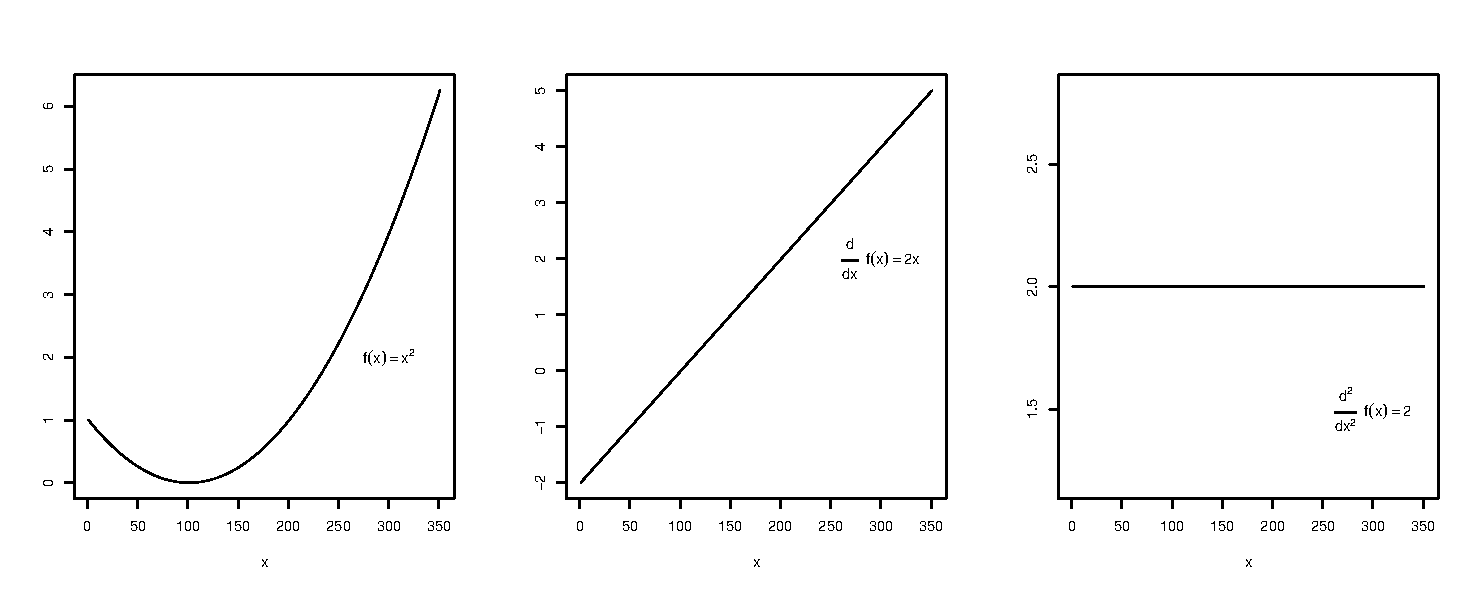
\includegraphics[width=6.5cm]{abb1.png}  % width legt Breite der Graphik fest

\begin{minipage}{0.8\linewidth}
\footnotesize{die Graphik sollte beschrieben werden, sodass man ohne den Text vorne zu lesen wei\ss{}, worum es geht: panel 1 zeigt die Funktion, panel 2 die erste Ableitung und Panel 3 die zweite Ableitung}
\end{minipage}

\end{figure}

\begin{figure}
\caption{titel der Graphik}
\label{fig:andereGraphik} \centering
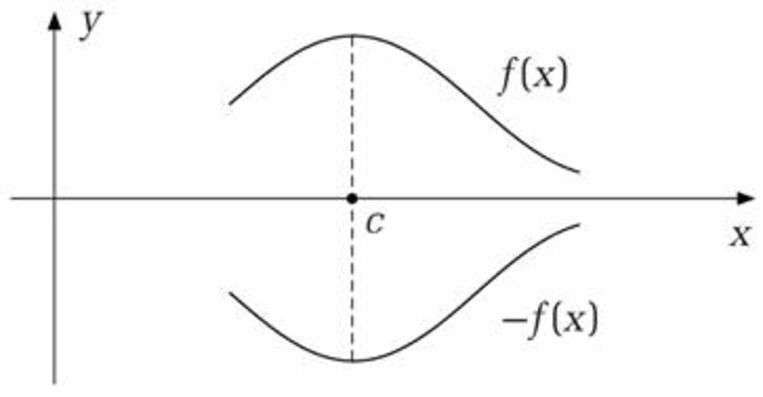
\includegraphics[angle=90,height=6.5cm]{abb2.jpg}  % angle dreht die Graphik, falls noetig; height legt die Hoehe der Graphik fest

\end{figure}

\begin{table}
\caption{Der Title der Tabelle}
\label{tab:Tabelle}
\centering
 \begin{tabular}{lc|r}
   Eine & kleine & Tabelle\\
\hline
   Text links & mittig & oder rechts \\
   & unterstrichen  & \\
\cline{2-2}
   \multicolumn{2}{c|}{\"uber zwei Spalten} & dritte Spalte \\
\end{tabular}   
\end{table}

   





\end{document}
